\subsection{Local weights and the identities they satisfy}\label{c4:local-tensors}

We begin with finite matrices. Their purpose is to encode paths on a
honeycomb cylinder in a form that permits us to exchange two column
parameters, remove a pair of columns, or fuse them into one. These operations
will determine the cylinder states by polynomial interpolation. The
parametrization comes from the dilute-loop Yang--Baxter weights
\cite{ZhouBatchelor1997,GlazmanManolescu2017}; we prove the identities needed
here, including their dependence on the loop-weight parameter.

The spin value $0$ records a vacant edge. The two values $+1,-1$ record the
two orientations of an occupied edge. These spins are algebraic labels:
scalar products below are bilinear and the transpose never conjugates a
coefficient.

Use a parameter \(\lambda\) near \(d_*=\pi/8\), and set
\[
 Q_\lambda=e^{i\lambda},\quad \chi=i e^{-2i\lambda},\quad n=\chi^2+\chi^{-2}=-2\cos(4\lambda),
 \qquad X_\lambda=\sin\lambda/\sin(2\lambda).
\]
At \(\lambda=d_*\) abbreviate \(Q=Q_{d_*},\ q=Q^2=\chi,\ x_*=X_{d_*}=1/(Q+Q^{-1})\); there \(n=0\).
Let $\mathcal H=\mathbb C^3$ with basis
\(\{|a\rangle:a=0,1,-1\}\). Tensor products carry the corresponding
product basis. Write \(c=\sum_{a=\pm1}\chi^a|a,-a\rangle,\ C=|00\rangle+c\); use \(c,C\) also as column maps from the trivial space. Define \(A|0\rangle=|00\rangle+X_\lambda c,\ A|a\rangle=X_\lambda(|a,0\rangle+|0,a\rangle)\) for \(a=\pm1\).

With spectral argument \(r=e^{ix}\) put
\[
 s_j=\sin(j\lambda),\quad a_j=\sin(j\lambda+x),\quad b_j=\sin(j\lambda-x),
 \quad p_0=s_2 s_3,\quad g(x)=a_2 a_3.
\]
Let $\operatorname{Swap}|a,b\rangle=|b,a\rangle$. The matrix
$B(r)$ acts on $\mathcal H\otimes\mathcal H$; when three factors are
present, $B_{12}$ and $B_{23}$ act on the indicated adjacent factors and
as the identity on the remaining factor. It has block \(uI+v\,{\rm Swap}\) when just one spin is occupied (nonzero), and on the remaining space in order (vacuum pair, both occupied) block
\[
 \begin{pmatrix} t & Uc^{\,t}\\ Uc & w I+W c c^{\,t}\end{pmatrix},
 \qquad
 (t,u,v,U,w,W)=(p_0+a_0 b_3,\ s_2 b_3,\ a_0 b_3,\ s_2 a_0,\ b_2 b_3,\ -a_0 b_1)/g(x).
\]
Here \(c\) in the block is restricted to both occupied, and \(t\) denotes the empty-cell weight (not a site variable). The identities below are meromorphic. \(B\) preserves total spin (charge), is transpose-symmetric and also invariant by simultaneous order reversal and charge negation. Under \(r\mapsto-r\) its entry \(B_{s,b;a,k}\) gains \((-1)^{|b|-|a|}=(-1)^{|s|-|k|}\) when nonzero. It is finite at \(0,\infty\); its other poles can only be at \(r^2=Q_\lambda^{-4},Q_\lambda^{-6}\), simple. At \(d_*\), \(a_5=b_3,a_6=b_2\), so \(t=1\) identically using \(a_2a_3=p_0+a_0a_5\). At \(r=Q_\lambda\) the weights divided by \(t\) in the indicated order are \(1,X_\lambda,X_\lambda^2,X_\lambda^2,X_\lambda^2,0\); at \(r=Q_\lambda^2\) they are \(1,X_\lambda^2,X_\lambda^2,X_\lambda,0,X_\lambda^2\). \cite{GlazmanManolescu2017,ZhouBatchelor1997}

The dilute braid--monoid setting is developed by Grimm and Pearce~\cite{GrimmPearce1993}. Their boundary-gauge distinctions are relevant here: the following scalar factors and cap conventions are part of the identities we prove.

\subsubsection{Crossing and inverse transport}

The two special ranks of $B$ are the reason for introducing $A$ and $C$.
Direct substitution gives \(B(1)=I,\ B(Q_\lambda^3)\propto C C^t,\ B(Q_\lambda^2)\propto A A^t\) (both proportionalities are equalities at \(d_*\)). Crossing reads
\[
 g(3\lambda-x)B_{23}(Q_\lambda^3/r)(C\otimes I)
   =g(x) B_{12}(r)(I\otimes C).
\]
Indeed at numerator level \(u\leftrightarrow U,\ w\leftrightarrow W\), while \(t,v\) stay. In entries one multiplies \(B(r)_{b,-k;-s,a}\) by \(\chi^{a-b}g(x)/g(3\lambda-x)\) to get \(B(Q_\lambda^3/r)_{s,b;a,k}\). This follows from the two blocks (e.g. a doubly occupied no-swap output with charges \(p,-p\) interchanges the numerators of \(w+W\chi^{2p}\) and \(W+w\chi^{2p}\); like charges interchange \(w\) and \(W\)).

Also \(B(r)B(r^{-1})=I\): the single block uses \(a_j b_j=s_j^2-a_0^2\), and \(w(r)w(r^{-1})=1\). On the cup/vacuum sector \(g(x)(w+nW)=p_0-a_0 a_3\) is the opposite \(t\) numerator since \(b_2b_3=p_0-a_0 b_5,\ b_5+n b_1=a_3\); the \(U\) numerators reverse sign. Here \(c^tc=n\), and
\((p_0+a_0b_3)(p_0-a_0a_3)-n s_2^2a_0^2=g(x)g(-x)\) by \(\sin(6\lambda)=(1-n)s_2\). For \(n\ne0\) split off the complementary doubly occupied space orthogonal to \(c\), then continue to \(n=0\). In particular
\[
\begin{gathered}
 B_{12}(r)B_{23}(Q_\lambda^3 r)(C\otimes I)=D(x)(I\otimes C),\\
 B_{23}(r)B_{12}(Q_\lambda^3 r)(I\otimes C)=D(x)(C\otimes I),\\
 D(x)=g(-x)/g(3\lambda+x).
\end{gathered}
\]

\subsubsection{Exchanging three adjacent columns}

The next identity ensures that moving a column past two others gives a
consistent result. For arbitrary spectral parameters $r,z$, as an identity
of meromorphic matrices on $\mathcal H^{\otimes3}$, it reads
\[
 B_{12}(z) B_{23}(rz) B_{12}(r)= B_{23}(r)B_{12}(rz)B_{23}(z).
\]
Equality at \(z=1,1/r\) follows by identity and unitarity. At \(z=Q_\lambda^3\) it follows by the two displayed \(C\)-transports and transpose, and at \(z=Q_\lambda^3/r\) by crossing on the range and on the transposed range of the middle rank-one insertion (the crossing scalars agree on the two sides). In more detail at the latter point the products up to common scalar read
\(B_{12}(Q_\lambda^3/r)(I\otimes C)(I\otimes C^t)B_{12}(r)\) and
\(B_{23}(r)(C\otimes I)(C^t\otimes I)B_{23}(Q_\lambda^3/r)\).
There is also equality at \(z\to0\). Indeed after a common scalar \(-e^{8i\lambda}\) the limiting \(B(z)\) is
\[
 |p,k\rangle\ \mapsto\ \xi^{pk}|k,p\rangle+(\xi-\xi^{-3})[p=1,\ k=-1]|1,-1\rangle,\qquad \xi=-e^{2i\lambda}
\]
by substitution. Two such leading transports move the initial third spin \(k\) to the first slot, with factor \(\xi^{k(S_1+S_2)}\) on the passed pair (\(S|p\rangle=p|p\rangle\)), plus for \(k=-1\) a term moving \(+1\) there instead and applying \((\xi-\xi^{-3})(L\otimes \xi^{-S}+\xi^S\otimes L)\), where \(L|1\rangle=|-1\rangle\), \(L=0\) on the other basis elements. These pair operators commute with \(B(r)\): the second is symmetric about vacancies, preserves occupancy and kills \(c,c^t\) on contraction by \(\chi\xi+(\chi\xi)^{-1}=0\). This verifies the claimed equality at zero. (At \(z\to\infty\) there is analogously a scalar \(-e^{-8i\lambda}\), weighted swap with \(\xi^{-1}\), and the opposite one-way flip.)

Now multiply the braid relation by \(z^4 g(y)g(x+y)\), \(z=e^{iy}\). Entries become polynomial of degree at most eight, of fixed parity by the sign rule (track the initial third site ending first). For generic \(r,\lambda\) the four finite nonzero test points and their negatives, together with zero, suffice, proving the identity.

\subsubsection{Fusion to a single spin}

The cup $C$ removes a pair of sites. The map $A$ instead replaces two sites
by one. The precise transport identities for this second operation are
\[
 \begin{aligned}
 B_{12}(r)B_{23}(Q_\lambda^2 r)(A\otimes I)&=d_f(x)(I\otimes A)B(Q_\lambda r),\\
 B_{23}(r)B_{12}(Q_\lambda^2 r)(I\otimes A)&=d_f(x)(A\otimes I)B(Q_\lambda r),\qquad d_f(x)=b_3/a_5.
 \end{aligned}
\]
Here \(D(x)=d_f(x)d_f(x+\lambda)\), both transport scalars being 1 at \(d_*\). The second equality follows from the first by unitarity (\(d_f(-x-2\lambda)=1/d_f(x)\)).

To verify the first, the braid identity places the output already in range \(I\otimes A\), using range \(B(Q_\lambda^2)={\rm im}\, A\). Read the components on slots \((s,0,b)\) there. Write primes and tildes on normalized weights for shifts \(+2\lambda,+\lambda\), respectively, \(X=X_\lambda\), \(d_f=d_f(x)\). The required scalar equalities are
\[
 \begin{aligned}
 d_f\tilde t&=t t'+n X U u',\\
 d_f\tilde u&=X(u t'+v u')=t u'/X+U(n w'+W'),\\
 d_f\tilde U&=u v'+v U'/X=X(t U'+U v'),\\
 d_f\tilde v&=v v'+X u U'=t v'+U U',\\
 d_f\tilde w&=u u'+v w',\qquad d_f\tilde W=v W'.
 \end{aligned}
\]
Indeed the last applied \(B\) contributes on rows \((0,0)\) as \(t\) or \(U\chi^p\) from \((p,-p)\), and on \((s,0)\), \(s\ne0\), as \(u,v\) from a single \(s\). Thus vacuum input, expanded first as \(|000\rangle+X\sum_p\chi^p|p,-p,0\rangle\), gives \(tt'+n X Uu'\) and the cup term with \(u v'+v U'/X\) after extracting the output \(A\). Double input expanded from \((p,k)\) as \(X(|p,0,k\rangle+|0,p,k\rangle)\) gives \(X(t U'+U v')\) on cup annihilation and \(u u'+v w',v W'\) on double propagation. The two single inputs similarly give respectively \(X(u t'+v u'),t v'+U U'\) from spin on slot one and \(t u'/X+U(n w'+W'),v v'+X u U'\) from spin on slot two.

For substitution drop normalizing denominators, replacing \(d_f\) by \(a_2 b_3\). The numerator lists at prime and tilde arguments in order \(t,u,v,U,w,W\) are
\[
 (p_0+a_2b_1,s_2b_1,a_2b_1,s_2a_2,-a_0b_1,a_2a_1),\quad
 (p_0+a_1b_2,s_2b_2,a_1b_2,s_2a_1,b_1b_2,a_1a_0).
\]
The \(U\) formulas use \(b_1+a_0/X=a_1\) and \(X[p_0+a_0(b_3+b_1)]=s_1s_3+a_0b_2=a_1b_3\); the \(v\) formulas use \(a_1b_2=s_1s_2+a_0 b_1\), \(s_3b_1+s_2 a_0=s_1 b_3\).

For \(u\) use \(X[p_0+(a_2+a_0)b_1]=a_2b_2\); the second expression with \(b_1/X=b_2-a_0\) uses \(-p_0-s_1s_2+b_2b_3-n a_0b_1+a_2a_1=0\). Finally for \(t\), use \(a_2 b_3=p_0+a_0 b_1\) and \(a_2 b_1=s_2s_1-a_0a_1\), reducing to \(s_3(b_3-a_1-b_1)=(1-n)s_1 b_1\). These all follow by elementary sine addition, and \(w,W\) immediately by \(a_2 b_2=s_2^2-a_0^2\). This finishes the tensor checks.

\subsection{Cylinder states and the physical transfer limit}\label{c4:cylinder}

We now place these matrices around a cylinder. There are two points to
establish before using a stationary state: the row operations must respect
noncrossing paths, and the stationary state at the positive honeycomb
weights must exist with a fixed normalization. We first define the row
algebra, then prove convergence through its path interpretation.

\subsubsection{Rows, twists, and fusion}

Take \(N\) spatial slots \(1,\ldots,N\) periodically, seam between last and first, twist \(\eta\ne 0\). With site parameters \(z=(z_1,\ldots,z_N)\), \(t_i=z_i^2\), define the open row \(M_{p,k}(z;u)\) by fixing \(s_0=p,s_N=k\) and summing over intermediate spins in
\[
 (M_{p,k})_{b;a}=\sum \prod_{i=1}^N B(z_i/u)_{s_{i-1},b_i;a_i,s_i}.
\]
(The \(u\) here is a spectral parameter.) Put \(T_\eta(z;u)=\sum_s\eta^s M_{s,s}(z;u)\), also \(T_\eta(\varnothing;u)=1+\eta+\eta^{-1}\). These closed transfers operate on total spatial charge zero and are rational in \(y=u^2\) by parity. Ordinary adjacent exchanges of the site list \(z\) intertwine \(T_\eta\), even each \(M_{p,k}\), via \(B_{i,i+1}(z_i/z_{i+1})\) from old to new order, by the braid relation. Rotation of \(z\) one slot left likewise intertwines \(T_\eta\) by
\(\Omega |a_1,\ldots,a_N\rangle=\eta^{a_1}|a_2,\ldots,a_N,a_1\rangle\)
by charge conservation. \(T_\eta(z;u)\)'s commute as \(u\) varies. Indeed for two auxiliaries (lower row \(u_1\), upper \(u_2\)) the site factor from ordered slots (spatial input, two incoming auxiliaries) to (two outgoing auxiliaries, spatial output) is \(K_i=B_{23}(z_i/u_2)B_{12}(z_i/u_1)\). The braid identity interchanges the auxiliary parameters by \(B(u_1/u_2)\), generically invertible and commuting with their combined twist, so their combined twisted trace is unchanged.

There are product identities at any site \(j\), writing \(e^{ix_{ij}}=z_i/z_j\):
\[
 \begin{aligned}
 T_\eta(z;z_j)T_\eta(z;Q_\lambda^{-2}z_j)
   &=\Big(\prod_i d_f(x_{ij})\Big)T_\eta(z;Q_\lambda^{-1}z_j),\\
 T_\eta(z;z_j)T_\eta(z;Q_\lambda^{-3}z_j)&=\Big(\prod_i D(x_{ij})\Big) I .
 \end{aligned}
\]
Indeed in the first case each \(K_i\) transports the auxiliary subspace \({\rm im}\,A\) by the second \(A\)-identity above, and \(K_j\) has output only into this subspace. Thus the trace restricts to it, with exactly the fused twist by charge, giving the first formula. Similarly use \(C\) for the second. At \(\lambda=d_*\), crossing gives on total charge zero
\[
 T_\eta(z;u)^t=T_{\eta^{-1}}(z^{-1};Q^{-3}/u)
\]
with site inverses in original order: cross at each \(B\), transpose the two-spin matrix (it is symmetric), and negate auxiliary spins; powers across sites cancel by total charge.

\subsubsection{Noncrossing pairings and loop weights}

The spin representation alone does not express self-avoidance. For that
purpose we keep the pairing of the occupied boundary slots. A
\emph{link state} is a noncrossing partial matching drawn below the cut of
the cylinder, with the winding class of every arc recorded. Slots not
matched are vacant. The following description makes the resulting
finite state space and its spin representation explicit. Lift the cylinder
to its periodic covering strip. Each lifted arc cuts off an interval \([i,j]\) with \(i<j<i+N\) on the cut: any larger separation would interlace with a translate. All translates of all intervals have noninterlaced endpoints. Include unpaired slots as vacancies and include the empty state. This is a finite formal basis. It maps linearly into spin tensors of charge zero by giving each arc independently spins \(s,-s\), \(s=\pm1\), at the indicated ends, summing with factor
\[
 \chi^s \eta^{k s},\qquad k=[\text{interval crosses the seam}].
\]
Call the range the link image (no injectivity assumed); the empty coefficient passes through unchanged. It transforms by \(\Omega\) for the above rotation. Ordinary projections testing vacancy or total occupancy at any given slots preserve the image.

The transfer rows \(T_\eta\) intertwine this map with spinless diagrammatic transfers, loop weights \(n\) for a contractible loop and \(\eta+\eta^{-1}\) for a winding one. To see the local choices, put \((a,k;s,b)\) at the
(bottom,right;left,top) ports of a square. Positive arrows point upward on
vertical edges and leftward on horizontal edges. The six unoriented local
weights are shown in Figure~\ref{a:local-cells}. Empty has weight \(t\); a bottom-left or right-top connection weight \(u\); a vertical or horizontal straight connection \(v\); a bottom-right or left-top connection \(U\); double connections of the first turn type have weight \(w\), of the second \(W\). The matrix sums these with an extra oriented factor along each strand
\(\chi^{-T/2+m_{\rm out}-m_{\rm in}}\), where \(T\) is signed turning in units of a quarter turn (round the diagrams), \(m_{\rm hor}-m_{\rm vert}=1/2\). Indeed bottom to left and right to top, and their reversals, have exponent zero, bottom to right and top to left exponent \(+1\), inverses \(-1\), as in the cup factors.

A lower boundary arc between vertical stubs has turn \(-2s\) by closing along its interval. Seam factors count signed left crossings. Both kinds of phases thus concatenate.

Contractible simple loops have turn \(\pm4\), essentials turn 0 and signed crossing number \(\pm1\). For the latter crossing count view the cylinder as a punctured plane and use the index of a Jordan loop; for turning concatenate arbitrarily many lifted periods starting at a highest point and close simply above their height by three segments, bounding the total turn independently of the number of periods. Summing free orientations gives the claimed loop weights, leaving again a link state.

\begin{figure}[tbp]
\centering
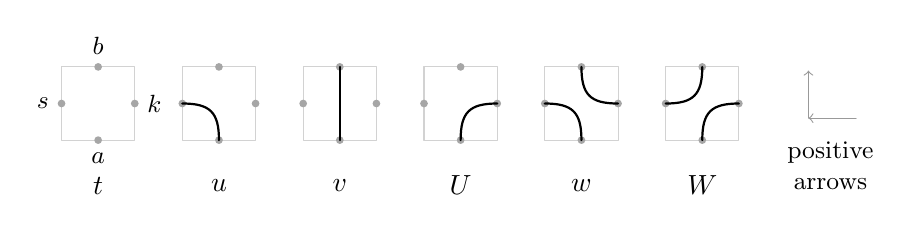
\begin{tikzpicture}[scale=.93,line cap=round,line join=round]
\foreach \j/\lab in {0/t,1/u,2/v,3/U,4/w,5/W} {
  \begin{scope}[shift={(1.65*\j,0)}]
  \draw[gray!35] (-.5,-.5) rectangle (.5,.5);
  \foreach \x/\y in {0/-.5,.5/0,0/.5,-.5/0}
    \fill[gray!70] (\x,\y) circle (1.5pt);
  \node at (0,-1.12) {$\lab$};
  \ifnum\j=0
    \node[below,font=\small] at (0,-.54) {$a$};
    \node[right,font=\small] at (.54,0) {$k$};
    \node[left,font=\small] at (-.54,0) {$s$};
    \node[above,font=\small] at (0,.54) {$b$};
  \fi
  \ifnum\j=1 \draw[thick] (0,-.5) .. controls (0,-.12) and (-.12,0) .. (-.5,0);\fi
  \ifnum\j=2 \draw[thick] (0,-.5)--(0,.5);\fi
  \ifnum\j=3 \draw[thick] (0,-.5) .. controls (0,-.12) and (.12,0) .. (.5,0);\fi
  \ifnum\j=4
    \draw[thick] (0,-.5) .. controls (0,-.12) and (-.12,0) .. (-.5,0);
    \draw[thick] (.5,0) .. controls (.12,0) and (0,.12) .. (0,.5);
  \fi
  \ifnum\j=5
    \draw[thick] (0,-.5) .. controls (0,-.12) and (.12,0) .. (.5,0);
    \draw[thick] (-.5,0) .. controls (-.12,0) and (0,.12) .. (0,.5);
  \fi
  \end{scope}
}
\begin{scope}[shift={(10,0)}]
  \draw[->,gray!80] (-.3,-.2)--(-.3,.45);
  \draw[->,gray!80] (.35,-.2)--(-.3,-.2);
  \node[font=\small,align=center] at (0,-.85) {positive\\arrows};
\end{scope}
\end{tikzpicture}
\caption{The six local connection weights in the row convention
\(B_{s,b;a,k}\). The first cell labels the bottom/right input ports
\(a,k\) and left/top output ports \(s,b\); positive arrows point upward
and leftward. A dot is a port; an unused port is vacant. For each
single-strand cell, its complementary pair of
ports has the same unoriented weight. Each strand may be oriented either
way, with the phase specified in the text. The two double-strand cells
are noncrossing.}
\label{a:local-cells}
\end{figure}


Local adjacent \(B\) acting on spatial slots also preserves the link image by the same diagram calculus drawn now with two bottom, two top vertical stubs and all other stubs propagating. Here \(u\) propagates a single occupied straight, \(v\) slides it past a vacancy, \(w\) propagates both, while \(U,W\) are cup/cap choices with factors \(c,c^t\) by the signed half-turns. Similarly \(C,A\) in insertion order across no seam and their transposes into the shorter spaces preserve link images (short cups/caps or vacant and single-spin propagation). In particular at \(\lambda=d_*,\eta=\pm i\), all loops have zero spinless weight and an exchange \(B\) preserves the all-empty coefficient on this image (also \(t=1\)).

\subsubsection{The honeycomb weights}

We have identified the loop weights in a finite row. We next identify the
positive physical specialization, where every occupied vertex has weight
$x_*$. At homogeneous \(z_i=1,\lambda=d_*,u=Q^{-1}\), diagram rows split each square into two trivalent vertices sharing an edge, carrying respectively the bottom-left and right-top ports. Each visited vertex contributes precisely \(x_*\) by the local weights, with at most one strand visiting it; these are honeycomb diagrams. More explicitly take \(h=(\sqrt3,0), v=(\sqrt3/2,3/2)\), vertices
\[
 P_{ij}=ih+jv,\qquad R_{ij}=P_{ij}+(h+v)/3
\]
(modulo horizontal period \(Nh\) on the cylinder); \(P_{ij}\) neighbors \(R_{ij},R_{i-1,j},R_{i,j-1}\). At \(u=Q^{-2}\) instead group bottom-right and top-left; the bases are \(h,v'=v-h\), and the pair displacement \(P'\to R'\) now \((v'-h)/3\), so the same honeycomb cylinder with a different grouping. The line between rows is a horizontal cut through perpendicular edges at their midpoints. Also at general nearby \(\lambda,u=Q_\lambda^{-1},z_i=1\), divide each cell by its empty weight to give the first honeycomb geometry with \(X_\lambda\) per visited vertex.

\subsubsection{A finite bound for boundary paths}

To pass from a finite-height cylinder to its stationary state, we require
an upper bound on the weight of each boundary arc. We derive it from the
honeycomb parafermionic identity of Duminil-Copin and Smirnov
\cite{DuminilCopinSmirnov2012}, with spin $5/8$. The same estimate also
controls crossings of a strip.

Take a bounded convex domain cut out along row-cut lines of the lattice and their rotated counterparts (by honeycomb symmetries); the boundary stubs are perpendicular edges ending at midpoints, never at corners. Fix a starting boundary midpoint \(o\). Sum over walks to edge midpoints \(p\), each walk visiting interior vertices self-avoidingly, changing edge at every vertex, depositing
\(x_*^{\#\mathrm{vertices}}\exp(-i\sigma\,{\rm wind})\), \(\sigma=5/8\), to \(F(p)\). Winding is the signed total turn in radians; include the trivial walk. At every vertex \(V\) inside, with neighboring midpoints as complex coordinates, we have
\[
 \sum_p(p-V)F(p)=0.
\]
Indeed an arrival without prior \(V\) from the edge side opposite \(V\) (including the trivial arrival if appropriate) groups with its two extensions through \(V\), by \(1+2x_*\cos((2+\sigma)\pi/3)=0\). The remaining arrivals from outside \(V\) to \(p\) have passed via \(q\to V\to r\) for the other two midpoints; pair with using \(q\to V\to p\) and the reversed excursion now ending at \(r\). The loop via \(r\) returning \(p\) closed back at \(V\) is simple with \(q\) outside (prefix from the boundary). For instance arrange \(q,r,p\) round \(V\) at angles \(0,2\pi/3,-2\pi/3\): that loop is positive and winding after the prefix adds \(5\pi/3-\pi/3=4\pi/3\), versus its negative for the partner. Their contributions cancel since \(\cos((2+4\sigma)\pi/3)=0\); reflection is identical.

Summing leaves only the boundary. Each path to another boundary midpoint has \(|{\rm wind}|\le\pi\) by closing from exit to entrance along the positively directed convex boundary (corner turns \(+\pi/2\) at each endpoint and intermediate boundary turn in \([0,2\pi]\)). Relative to the initial inward step the real parts thus contribute at least \(\cos((1-\sigma)\pi)\) times masses after dividing by half-edge length, while the \(o\) term contributes \(-1\). Exhausting a half-plane or strip by such convex polygons now bounds, by an absolute constant, the total \(x_*\)-mass of boundary arches from a given boundary midpoint in that half-plane, or bridges from a boundary midpoint reaching the parallel other boundary in the strip.


The honeycomb connective-constant theorem
\cite[Theorem~1]{DuminilCopinSmirnov2012} gives, for the number $c_m$ of
$m$-edge walks from a fixed vertex,
\[
 \mu=\lim_{m\to\infty}c_m^{1/m}=\sqrt{2+\sqrt2},\qquad x_*=\mu^{-1}.
\]
Consequently $x_*$ is the convergence radius for these edge-counted walks.
The boundary estimate also yields a quantitative upper bound by the
successive-extrema unfolding principle~\cite{HammersleyWelsh1962}; we give
the argument, including its lattice endpoint conventions.

For completeness, the boundary estimate itself implies that $x_*$ cannot
exceed the plane convergence radius. The endpoint conversion is also
needed in the quantitative estimate, so we give its details. Put \(Y=2\,({\rm vertical\ height})\); increments are nonzero integers of magnitude at most 2. For walks from a given vertex at one \(Y\)-extremum to their other extremum of specified \(Y\), confined between them (strictness not needed, span nonzero), the total \(x_*^{\#\mathrm{edges}}\) is uniformly bounded: extend to perpendicular cut midpoints just below and above the two extreme rows. At the minimum attach first a neighboring lower \(P\) if at an \(R\), and at the maximum a neighboring higher \(R\) if at a \(P\), by fixed conventions. Added vertices lie strictly outside the old heights, and the bridge bound applies with only bounded length adjustment. An arbitrary \(m\)-step walk splits at a lowest vertex. Along each arm going away, cut at the last highest vertex, then last lowest of the remainder, alternately until the end. The positive spans are decreasing strictly after a possible initial equality, and sum to at most \(2m\). Thus the original chronology is a concatenation of \(O(\sqrt{m})\) extremum-to-extremum bridges, some reversed back, with at most \((C m)^{O(\sqrt{m})}\) possible signed span lists. Multiplying the uniform bounds gives subexponential total \(m\)-step mass at \(x_*\). The matching opposite radius bound will also follow from the winding masses below.

In the notation just introduced, the quantitative conclusion is
\begin{equation}
 c_mx_*^m\le \exp\!\bigl(C\sqrt m\log(m+1)\bigr)
 \qquad(m\ge1),                                      \label{c4:unfolding}
\end{equation}
for an absolute constant $C$.  For each extremum-to-extremum bridge in
this decomposition, the extension adds $a,b\in\{0,1\}$ vertices at its
lower and upper ends.  An $l$-edge bridge therefore has port weight
$x_*^{l+1+a+b}$; the exterior half-edges add no visited vertices, and
inverse multiplicity is bounded.  These conversions preserve the uniform
piece bound used in the unfolding count.

\subsubsection{Existence and uniqueness of the normalized stationary state}

Return to a cylinder of fixed circumference $N$. The boundary-path bound
now proves convergence of the row iteration, rather than merely bounding
its matrix entries. At either homogeneous physical transfer,
\(\eta=\pm i\), consider the formal matching matrix at \(d_*\). It is nonnegative, loops killed. Its powers on the empty state increase coefficientwise since all-empty propagation is available. They are bounded: each remaining arc lifts to a planar arch in the lower half-plane from a given slot; a product of the just-proved bounds dominates each coefficient. Every nonempty matching \(J\) is reachable with positive coefficient: build one periodic arc at a time in decreasing interval length, extending already present ends vertically. No already occupied slot lies in the new intervals by noninterlacing. In one row a top-to-top arc can run horizontally between its two slots with positive allowed turns, simultaneously with the required vertical passes outside. Writing $T$ for the matching transfer, for each $J\ne\varnothing$
there are $m\ge1$ and $\epsilon>0$ such that
$T^m e_\varnothing\ge e_\varnothing+\epsilon e_J$ coefficientwise.
Consequently
\[
 0\le \epsilon T^n e_J
 \le T^{n+m}e_\varnothing-T^n e_\varnothing\longrightarrow0.
\]
Thus every nonempty basis vector is sent to zero in the limit. This gives a rank-one projection limit on the formal space (eigenvalue \(1\) simple, all others of modulus less than 1). Hence also on its spin image, with unique fixed vector normalized to empty coefficient 1 and obtained from vacuum by the transfer limit. At fixed \(\lambda=d_*,\eta=\pm i\), varying sites near homogeneous and fixing the auxiliary at a physical value, that simple normalized link eigenvector continues regularly with eigenvalue 1 (the empty coefficient of transfer is unchanged on this image). In particular uniqueness there also implies generic uniqueness if supplied with a rational normalized eigenvector.

\subsection{Polynomial formulas for the two stationary states}\label{c4:vacua}

The stationary states just obtained by a positive transfer limit have
rational continuations in the column parameters. We construct those
continuations explicitly. The two twists $i$ and $-i$ require different
polynomial degrees; both will be needed because adding their marked
observables retains winding polygons and cancels contractible polygons.

Throughout this subsection \(\lambda=d_*\). We use \(p=2,\eta=i=q^2\)
and \(p=1,\eta=-i=q^{-2}\), respectively. Put \(P=2+\sqrt2,\ K_2=P q^3,\ K_1=1+q^3\). For each choice we construct a polynomial vector $V_N(z)$ in the link
image, with \(V_0=1\) and \(V_1=|0\rangle\). When both constructions occur
in one formula, their choice is specified by $p$ or by the twist $\eta$.
The defining requirements are as follows:

\par\noindent\textbullet\quad Homogeneous \(z\)-degree \(p N(N-1)\). Each component on spins \(s_l\), divided by \(\prod_l z_l^{|s_l|}\) (called stripping), is polynomial in the \(t_l=z_l^2\), of degree per \(t_l\) at most \(p(N-1)-|s_l|\).
\par\noindent\textbullet\quad Exchange of adjacent arguments \(z_i,z_j\) (in order before exchange) acts by \(B_{ij}(z_i/z_j)\); rotation left acts by \(\Omega\).
\par\noindent\textbullet\quad For spin 0 at \(l\), the value at zero and the leading scale at infinity in \(t_l\) are respectively \(\prod_{k\ne l}t_k^p\) and \(t_l^{p(N-1)}\) times \(V_{N-1}\) with \(l\) removed.

Polynomial exchange equations and special-parameter reductions have
counterparts in other loop models. Garbali and Nienhuis study polynomial
exchange equations and fusion recurrences for dilute $O(1)$ ground states,
with determinant formulas for the associated sum
rules~\cite{GarbaliNienhuis2017Ground,GarbaliNienhuis2017Sum}. Here the loop
weight is zero, and both normalized vectors are constructed by the
interpolation argument below.

\subsubsection{Pair values and the two-site initial condition}

The degree and endpoint requirements do not by themselves determine
$V_N$. We prescribe its values when two column parameters have the cup
ratio. We impose pair prescriptions at \(z_j=Q^3 z_i\). For \(p=2\) prescribe one for every directed pair \(i\to j\) in the cyclic list. For \(p=1\) only require \(i<j\). First for an order \((\ldots,i,k_1,\ldots,k_r,j,\ldots)\), insert \(C\) at \(i,j\) made adjacent (just before the intermediate list) on \(V_{N-2}\) of the other sites, then transport \(j\) right to its specified position over the intermediate list by successive exchanges \(B(z_j/z_{k_l})\). Multiply by
\[
 \Pi_{ij}=K_p u^p\!\!\prod_{k\ne i,j}[(t_k-q^{-3}u)(t_k-q^6 u)]^p,\qquad u=t_i.
\]
Call the result \(W_{ij}\). For a cyclic prescription in construction \(p=2\), rotate to this situation (cut outside the directed interval) and rotate the result back by the inverse powers of \(\Omega\). The choice of linearizing cut does not matter using cyclicity of the smaller tensor: a block rotated over the cut when comparing two choices either misses this operation or contains the entire affected block, which conserves the total spin of its spectators; also \(\Omega^N=I\) on charge zero. These prescriptions respect site parity under stripping (including simultaneous signs at paired endpoints); this follows by the sign rule for exchanges and equal starting occupancies at the two ends of \(C\).

At \(N=2\) write \(V_2=D|00\rangle+H c\). Use
\[
 \begin{array}{c|cc}
 &D&H\\\hline
 p=2&t_1^2+(2+2\sqrt2)t_1t_2+t_2^2&P Q^3 z_1 z_2(t_1-t_2)/(1-q^3)\\
 p=1&t_1+t_2&(Q^3+Q^{-3})z_1 z_2 .
 \end{array}
\]
Indeed \(c^tc=0\); exchange sends \(H\) to \(U D+wH\), equal to \(-H,H\) respectively. By the weights at \(z_1/z_2=e^{ix}\), the ratios needed are
\(-U/(1+w)=-s_2\sin x/(\cos d_*+\cos(3d_*)\cos(2x))\) and \(U/(1-w)=s_2/(2s_3\cos x)\), giving the table. Rotation of \(c\) contributes scalar \(-1,1\) respectively. The prescribed adjacent pair values and other constraints now follow directly.

\begin{proposition}[The two polynomial vacua]\label{prop:polynomial-vacua}
For each of the choices \((p,\eta)=(1,-i),(2,i)\), there is a unique
polynomial family \(V_N\), \(N\ge0\), satisfying the degree, exchange,
rotation, deletion, and pair requirements above. It lies in the link
image, its empty coefficient \(D_p=V_N^{\rm empty}\) is not identically
zero, and
\[
                     T_\eta(z;u)V_N(z)=V_N(z)
\]
as a rational identity for every auxiliary parameter \(u\).
The normalized rational vector \(V_N/D_p\) extends regularly to
homogeneous sites and there equals the empty-normalized stationary state
obtained from either physical transfer limit.
\end{proposition}

\subsubsection{Compatibility of the pair prescriptions}

We prove Proposition~\ref{prop:polynomial-vacua} by induction in \(N\),
starting with the displayed initial vectors. The first step is to check
that the prescribed values agree wherever two pair slices meet.
All parameters not constrained by those slices are first taken
generic. Meromorphic continuation will then cover every regular
specialization. Each \(W_{ij}\) is covariant by ordinary adjacent swaps not swapping its two endpoints together. For endpoint \(j\) this follows by its transport definition and unitarity; for \(i\) moving past a slot \(k\) use
\(B_{12}(z_k/z_i)(I\otimes C)=B_{23}(z_j/z_k)(C\otimes I)\), or reverse by unitarity. For spectator swaps use smaller-tensor exchanges and the braid relation if both spectators lie on the transport route. For a cyclic interval one can linearize across a cut outside the route not splitting the swap (moving a cut past a whole swapping block is compatible by charge); the prescriptions are also covariant by rotation for \(p=2\).

It follows that evaluations from two disjoint prescribed pairs at their intersection agree: place both pairs positive-adjacent without swapping the endpoints of either together, and apply smaller-tensor prescriptions and commuting insertions. In the cyclic case one may migrate an end around over other labels up to adjacency (the second pair can cross the whole first block this way) and rotate both away from the seam. The products of prefactors agree: for start parameters \(u,v\) the extra cross factor before power \(p\) is \(q^6\prod_{k=\pm2,\pm3}(v-q^k u)\), symmetric. All swaps of unrelated labels here are generically invertible.

At two pairs with common start (so equal ends), arrange the triple consecutively preserving the orientations; transporting one equal end past the other uses \(B(1)=I\). For common end, similarly use \(B_{23}(Q^3)(C\otimes I)=I\otimes C\); again values agree. At a chain intersection \(i\to j\to k\) both evaluations vanish: \(\Pi\) has an order-\(p\) zero at the third parameter, with at most one exchange pole there; when \(p=1\), \(i<j<k\) and the third parameter in either prescription is outside its transport route, so not a pole at all.

\subsubsection{Interpolation and polynomial degree bounds}

Assume that the smaller tensors have been constructed. We now construct
$V_N$, check that the apparent interpolation poles cancel, and prove its
bounds in every parameter. For \(N\ge3\), interpolate after stripping in
\(t_N\). Use nonzero nodes
\[
 r_{i\epsilon}=q^{3\epsilon}t_i,\qquad i<N,\quad
 \epsilon\in J_p,\qquad J_1=\{1\},\ J_2=\{1,-1\}
\]
by those prescriptions (\(z_N=Q^{3\epsilon}z_i\)), and also zero with the required deletion input if \(s_N=0\). With \(\rho=[s_N=0]\), the Lagrange factors for nonzero nodes are
\[
 L_{i\epsilon}=(t_N/r_{i\epsilon})^\rho
       \prod_{(a,\gamma)\ne(i,\epsilon)}\frac{t_N-r_{a\gamma}}{r_{i\epsilon}-r_{a\gamma}} .
\]
Use \(L_0=\prod_{a,\gamma}(1-t_N/r_{a\gamma})\) when needed. Homogeneity and charge zero hold, and the result unstripped stays in the link image since the extra scaling and interpolation weights depend only on occupancy at \(N\). Each prescribed input \(W\) is polynomial on the paired slice after stripping: every transport pole divisor involving the paired parameter and a spectator is canceled by \(\Pi\); at spectator zero the matrices stay bounded and parity suffices to strip, at simultaneous endpoint zero even the \(u^p\) supplies divisibility. Its stripped spectator degree has the desired bound since \(\Pi\) adds \(2p\) there, the raw smaller tensor grows by at most degree \(p(N-3)\), and bounded exchange and stripping then give the bound by parity (rounding down to integral degree).

Potential interpolation poles at coincident nonzero nodes from \(t_i=t_l\) cancel between the corresponding simple Lagrange poles by common start/end compatibility, and at \(t_i=q^{\pm6}t_l\) for \(p=2\) by chain vanishing. At \(t_l\to0,\infty\) for \(l<N\), the special terms \(i=l\), including stripping and Lagrange factor, grow respectively at worst as
\[
 O(t_l^{\,1-(|s_l|+|s_N|)/2-\rho}),\qquad
 O(t_l^{\,p(N-1)-(|s_l|+|s_N|)/2-\rho});
\]
indeed the raw paired input has bounds from \(\Pi\) of powers \(p,\ p(2N-3)\), and the other factors of \(L_{l\epsilon}\) beyond \((t_N/r)^\rho\) contribute at worst powers \(-(p-1),-p(N-2)\). These bounds have no pole and give the required degree (round by parity), subleading at infinity for vacant \(l\). In other terms use the spectator bounds and the zero input factor \(t_l^p\) canceling the \(L_0\) pole. Thus all coefficients are polynomial after stripping with the claimed degrees.

\subsubsection{Deleting a vacant spectator}

We have a polynomial vector with the required degrees. To complete the
induction, its deletion limits must agree with the smaller tensors in
every variable, not just in the interpolation variable. Fix a spectator
\(l<N\) with \(s_l=0\). At infinity, in nonspecial pairs only the smaller-tensor vacant \(l\) can contribute to the leading scale; if crossed it is passed exactly by the extreme swap. Thus these give \(t_l^{p(N-1)}\) times smaller interpolation terms (power \(2p\) from \(\Pi\) and \(p(N-3)\) from the smaller-tensor deletion, removed Lagrange factors tending to 1); the zero term likewise, special terms subleading as above.

At zero the nonspecial inputs scale to smaller inputs times \((\prod_{k\ne l,N}t_k^p)r_{i\epsilon}^p\), since the dropped spectator factors in \(\Pi\) give \(q^{3p}u^{2p}\); their extra Lagrange factors tend to \((t_N/r_{i\epsilon})^p\). These yield the nonzero-node terms needed after deletion. Special terms vanish if \(s_N\ne0\). Suppose \(s_N=0\) and write \(L'_0\) for the smaller zero basis. For \(p=2\) the special raw inputs before stripping at leading order are
\[
 P q^{3\epsilon} t_l^2 \!\!\prod_{k\ne l,N}t_k^4\, V_{N-2},
\]
as both endpoints remain vacant and the traveling end swaps exactly at leading order. Rotations if needed here and for spectator deletion do not pick up a phase from crossed vacancies. Multiplication by \(L_{l\epsilon}\sim t_N^2L'_0/[q^{3\epsilon}(q^{3\epsilon}-q^{-3\epsilon})t_l^2]\) gives cancellation. The ordinary zero input then yields the required zero term using the smaller-tensor deletion \((L_0\sim (t_N/t_l)^2L'_0)\). For \(p=1\) the special raw input is similarly at leading order
\((1+q^3)t_l\prod_{k\ne l,N}t_k^2 V_{N-2}\), with \(L_{l+}\sim t_N L'_0/(q^3 t_l)\), while the zero input has leading raw \(t_l\prod_{k\ne l,N}t_k^2 V_{N-2}\), with \(L_0\sim-t_N L'_0/(q^3t_l)\). These combine to exactly the desired zero term. Stripping spectator factors is common to all of these comparisons. This proves both deletion limits for \(l<N\); vacant \(t_N=0\) is already a node.

\subsubsection{All pair values, exchanges, and rotation}

The degree bounds and spectator deletions now let us test the remaining
identities by interpolation. First impose every required pair
\(i\to j\) not involving \(N\) by comparing as polynomials in spectator \(t_N\) on the slice. At the same nonzero interpolation nodes (still distinct generically), compatibility gives equality, and at zero if vacant use spectator deletion in \(W_{ij}\) by the same \(\Pi\), smaller-tensor and extreme-swap rules. Degree in \(t_N\) after stripping then proves the prescription.

For \(p=1\) deduce now the vacant infinity deletion at \(N\) as well: the difference in the leading coefficient from the required one, stripped, has all factors \(t_j-q^3t_i,\ i<j<N\), by the pair prescriptions and smaller-tensor infinity limit. Its total degree is at most \((N-1)(N-2)/2\), strictly less for any nonvacuum spin list. For the all-vacant component use also \(t_l=0\) for some \(l<N\) (the deletion limit there with smaller-tensor infinity gives agreement). Thus the difference vanishes.

Exchanges for either construction follow by testing a third label's parameter (\(N\ge3\)). At all pair nodes involving that label the pair covariances apply (its order relative to the partner is unchanged if \(p=1\)); at zero for a vacant spin use deletion. These suffice by degree since the exchanged sites are external to the variable being tested. Similarly for \(p=2\) test any label's parameter to show rotation using the cyclic covariances of the prescriptions and zero deletion. This also gives the remaining infinity deletion at \(N\) for \(p=2\).

Only rotation for \(p=1\) remains. Its pair prescriptions were imposed in
linear order, so cyclic covariance is not already available.
Consider the difference between \(V_N\) at the left-rotated list and
\(\Omega V_N\). All ordered pair specializations among labels
\(2,\ldots,N\) vanish by smaller-tensor cyclicity (the pair transport
misses slot 1); the vacant deletion limits for these labels vanish too
(difference at the specified leading scales). Thus any component vacant
at one of \(2,\ldots,N\) vanishes identically using \(N-2\) pair roots
there, zero and the infinity coefficient. The difference is supported on
that tail all occupied, and exchanges by \(B\) on the tail by what was
just proved. Projecting an exchanged adjacent pair to \(00\) forces
\(c^t\) annihilation there; hence the exchange acts by scalar
\(w(z_i/z_j)\) alone. Its poles now force both factors
\(t_j-q^2t_i,\ t_j-q^3t_i\) in the stripped polynomial for every
\(2\le i<j\le N\), by bringing these arguments adjacent (other generic
swaps nonsingular); the \(w\) numerator is nonzero generically there.
This exceeds the degree \(N-2\) per occupied variable since \(N\ge3\).
Hence rotation holds. We have finished the induction for both
constructions. Uniqueness follows from the same interpolation nodes and
degree bounds at each induction step.

\subsubsection{The empty component and the transfer fixed vector}

It remains to normalize the constructed vector and identify it with the
physical stationary state. Write \(D_p=V_N^{\rm empty}\), the coefficient
of the all-vacant spin tensor. It is symmetric by exchanges and link loop killing. In fact with \(X=(t_i)\)
\[\begin{gathered}
 D_2(X)=P^N\!\prod_{i<j}\left[\frac{p_K(t_i,t_j)}{t_i-t_j}\right]^2 \det[k(t_i,t_j)],\\
 p_K(x,y)=x^2+\sqrt2xy+y^2,\quad k(x,y)=xy/p_K(x,y).
\end{gathered}\]
Indeed this expression is polynomial (all \(p_K\) poles canceled and a Vandermonde zero in each of rows and columns). It has both required endpoint limits by inspection (in particular correct maximum degree). At \(t_j=q^3u,\ u=t_i\), the double pole term \(-k(u,t_j)^2\det k_{\rm red}\) in the determinant gives exactly \(\Pi_{ij}\) times the smaller formula: \(-P^2 q^6/(1-q^3)^2=P q^3\) and the extra spectator factors reduce by factoring \(p_K\). These and the vacant zero input suffice by interpolation since the constructions of \(W\) preserve the inserted empty coefficient apart from \(\Pi\). The inversion formula \(D_2(X^{-1})=\prod_i t_i^{-2(N-1)} D_2(X)\) follows. We do not need an analogous determinant here for \(D_1\). Both denominators are generically nonzero, also on slices of a pair at ratios \(q^{\pm1,\pm2,\pm3}\) (meaning either sign in any of the three powers), by deletion down to the displayed two-site components.

We next prove the fixed-vector identity
$T_\eta(z;u)V_N(z)=V_N(z)$ for every auxiliary parameter $u$, as a rational
identity. This is the step connecting the interpolation construction to
the transfer limit. Induct using one site variable \(t_l\); clear its two transfer pole factors and strip its output-spin parity. The difference has degree at most \(p(N-1)+2-|b_l|\) at output spin \(b_l\), by bounded extremes and rounding as before. It vanishes at the \(p(N-1)\) prescribed pair nodes involving \(l\), by \(W\), placing the pair adjacent and using \(C\)-transparency and smaller transfer (intertwining the swaps/rotations). At zero if \(b_l=0\) use deletion and extreme swap. It also vanishes at \(t_l=u^2\) and \(t_l=q^3u^2\) for auxiliary \(u\). Indeed put the site last in the first case \(z_l=u\): \(B(1)\) identifies \(s_{N-1}=a_N,\ s_0=s_N=b_N\) in row notation. The exchanges in the remaining row move the last argument left through all to the first position; the twist factor \(\eta^{b_N}\) undoes this rotation.

In the second case put the site first with \(z_1=Q^3u\); \(CC^t\) forces \(s_0=-b_1,\ s_1=-a_1\) with factor \(q^{a_1-b_1}\). Cross the remaining
\(B(z_i/u)_{s_{i-1},b_i;a_i,s_i}=q^{a_i-b_i}B(z_1/z_i)_{b_i,-s_i;-s_{i-1},a_i}\).
Phases cancel by charge, and this braid moves the first argument right to last while the twist again undoes rotation. The node count is sufficient (start the induction at \(N=0\)).

Set \(\Psi_\eta=V_N/D_p\); we call this normalized stationary vector the
\emph{vacuum}. These normalized rational vectors are regular by continuation at homogeneous sites and give exactly the physical transfer limits: even if a denominator representation vanishes there, generic uniqueness near those sites identifies the rational function locally with the regular link eigenvector already established. All exchanges/rotation, endpoint deletions with vacuum normalization (nonvacant outputs vanishing by the degree bounds), spin parities and transfer fixed identities thus hold in the stated limits or as rational identities.
This completes the proof of Proposition~\ref{prop:polynomial-vacua}.

\subsection{A marked row and its polygon interpretation}\label{c4:marked-row}

A closed transfer kills every loop when $\eta=\pm i$. To retain one loop,
we fix the orientation of a single auxiliary edge instead of summing it.
The resulting scalar has opposite signs on contractible polygons for the
two twists. We will first establish its finite algebraic properties and
then compute those signs geometrically.

Set \(\lambda=d_*\) and \(\eta=\pm i\). For an operator $H$ on the
$N$-site spin space, use the normalized rational vectors just constructed
to define the bilinear bracket
\[
 \langle H\rangle=\Psi_\eta(z^{-1})^t H\Psi_\eta(z),\qquad
 Z_\eta(y)=\langle M_{-,-}(z;\sqrt y)\rangle.
\]
Here $z^{-1}=(z_1^{-1},\ldots,z_N^{-1})$, and the symbols $-$ in
$M_{-,-}$ mean the auxiliary spin $-1$ at both ends of the open row.
Write \(P_{l,s}\) for the projector to spin \(s\) at site $l$.

\subsubsection{Normalization and pair reductions}
 One has \(\langle I\rangle=1,\ \langle P_{l,+}+P_{l,-}\rangle=0\): gluing two link states, read the bra as arcs \emph{above} with inverse twist (the arc turning and factors in its coefficients then have exactly the indicated signs). For a loop with signed left seam crossings \(N_L,N_U\) below and above respectively, the twist factor is \(\eta^{N_L-N_U}\), real (\(\pm1\)) if contractible and imaginary (\(\pm i\)) if essential, since \(N_L+N_U=0,\pm1\) respectively. The free orientations thus sum to zero by the turning phases. Occupancy restriction does not interfere, and the all-vacant coefficients are normalized.

By exchanges, transpose symmetry, unitarity and row intertwining, \(Z_\eta\) is symmetric in the site labels, rational in the \(t_i\) and \(y\) by the sign rule and site parity. In \(y\) poles can only come from \(\prod_i(y-q^2t_i)(y-q^3t_i)\), and both endpoints \(0,\infty\) give 1 since the weighted extreme swaps have total spatial charge zero, the scalar on each is 1 and one-way flips cannot restore the fixed auxiliary. Also sending a spectator \(t_k\) alone to either endpoint decouples that site, by the vacant leading limits of the vectors in both factors of the brackets and the extreme swap past a vacancy. At \(a=t_l\) one has the crossing value
\[
                         Z_\eta(a)=Z_\eta(q^{-3}a).
\]
Indeed put \(l\) last at \(y=a\); \(B(1)=I\) forces its output spin equal to the traced seam spin. Thus \(M_{-,-}\Psi_\eta=\eta P_{\rm last,-}\Psi_\eta\) by projecting \(T_\eta\Psi_\eta=\Psi_\eta\). At \(y=q^{-3}a\) put \(l\) first and \(B(Q^3)=CC^t\) similarly gives \(\eta P_{\rm first,+}\Psi_\eta\). Rotating both ket and bra from first to last multiplies the charged projector contractions by \(\eta^{2(\pm1)}=-1\); use the projector-sum vanishing.

Pair reductions hold rationally for otherwise generic variables, including generic \(y\): two site parameters \(t,q^2t\) replace by the single \(qt\), and \(t,q^3t\) delete. Arrange them ordered adjacent (across no seam) and use positive root ratios \(z_j/z_i=Q^2,Q^3\) respectively. The vacuum denominators in either order and either set of inverse arguments are nonzero generically on these slices by the decoupling limits down to the size-two vacua. In positive order the exchange \(B(Q^2)=A A^t\) or \(B(Q^3)=C C^t\) from reverse order places \(\Psi_\eta\) in the inserted image. Extract \(A\) or \(C\) by its left inverse. The result stays in the link image (\(A^t A\) diagonal \(1,2x_*^2,2x_*^2\), inverse just occupancy scaling, \(C^t C=1\)), has empty coefficient 1, and is a transfer fixed vector on the fused/deleted list by the spatial \(A,C\) transports, hence the corresponding shorter vacuum by generic uniqueness there.

In inverse-site arguments the order is opposite: exchange to positive order uses \(A A^t\) or \(C C^t\) on \(\Psi_\eta(z^{-1})\). By the result for positive order and injectivity, applying the transposed insertion alone thus yields exactly the shorter inverse vacuum. The same spatial transport identities hold in the open row, proving the pair reductions after contraction.

\subsubsection{The sign of a marked polygon}

We can now interpret the marked scalar at physical weights. The algebraic
states are complex, but the $-i$ marked observable will be a sum of
positive polygon weights. At homogeneous sites interpret
\(Z_\eta(q^{-k})\), \(k=1,2\), by surrounding the open row with the same physical rows (\(u=Q^{-k}\)) but twist \(\eta\) below and inverse twist above, vacuum on the two outer cuts, taking height limits. This gives the brackets by the transfer convergence and the crossed transpose identity. Draw first in oriented square topology as before, seam vertical. The right arrow fixed by the mark at its seam edge singles out a loop. All others sum to zero as before. Twist crossings of the marked loop now exclude the single marked crossing, and still use \(\eta^{N_L-N_U}\).

If contractible positive (counterclockwise), just before that right arrow on the seam upwards one is outside the loop, and just after one is inside; \(N_L=0,N_U=1\). For the negative loop \(N_L=1,N_U=0\). The two possible full phases are \(q^{-2}\eta^{-1}\) and \(q^2\eta\), both \(-1\) at \(\eta=i\), \(+1\) at \(-i\).

For net rightward essential, the point just before is in the bottom component and \(N_L=N_U=0\); for net left it is in the upper component and \(N_L=N_U=1\). Indeed crossings toggle sides, right arrows entering the left side of the oriented strand, and the net sign over the full seam records which component is which. Both essential phases are 1.

Similarly \(Z_\eta(1)=\eta\langle P_{\rm last,-}\rangle\) can use \(u=Q^{-1}\) on both sides, marking a downward arrow and a seam just to its right (the point on the cut there is thus on the left side of the arrow). For counterclockwise contractible \(N_L=-1,N_U=1\); for clockwise both 0, giving the same signs with the extra \(\eta\). For net right essential \(N_L=-1,N_U=0\); for net left \(N_L=0,N_U=1\), again total phase 1 including \(\eta\).

Consequently each marked value at minus twist counts both essential and contractible self-avoiding polygons through its edge with weight \(x_*^{|\gamma|}\) (\(|\gamma|\) the length), and at plus twist essential minus contractible. These statements pass to the limit since the minus sign choice of \emph{twist} made both sums positive and their limiting bracket finite. The orientation of the marked loop is uniquely fixed. The three edges for \(1,q^{-1},q^{-2}\) sample exactly one of each honeycomb edge type up to lattice translations, on the same cylinder: the first two are across vertical and horizontal diagram ports of the first grouping (\(h,v\)); the third is across a horizontal port of the second (\(h,v-h\)), hence an internal pair edge of the first.

\subsection{Finite identities for marked polygon masses}\label{c4:color-sum}

The marked-row interpretation reduces the winding mass to two finite
scalar calculations. The first computes the sum of all polygon masses
through one edge of each type. The second expresses the winding part as
a ratio of finite color sums. All identities are proved with generic
column parameters and then continued to the homogeneous cylinder.

Write \(d=q+q^{-1}=\sqrt2,\ P=2+d,\ c_*=2-d=2/P\). Use site list \(X=(t_i)\) and \(a\in X\) a distinguished parameter. Set
\[
 S'_{\eta,a}= Z_\eta(a)+ Z_\eta(q^{-1}a)+ Z_\eta(q^{-2}a),\qquad S_a=c_*+S'_{i,a}
\]
(where \(i\) in the twist denotes \(\sqrt{-1}\)). All unspecialized parameters in residue arguments are otherwise generic.

For a spectator \(b\), possible row poles of \(S'\) beyond vacuum denominators are \(b/a=q^{3,4,5,6}\). At \(q^3,q^5\) those collisions do not give poles: on the slice, the colliding \(y\)-residue of \(Z(y)\) vanishes by pair deletion, with that pole branch simple and disjoint from other \(y\)-poles and vacua regular generically. This gives boundedness when approaching in \(b\) with \(y\) fixed. At \(b=q^2 a\) there is no collision, and \(S'\) takes the shorter value at the fused mark \(q a\) by pair reduction and crossing there. At \(b=q^{-2}a\) the same holds with fused mark \(q^{-1}a\) by replacing \(Z(a)\) by \(Z(q^{-3}a)\) via crossing \emph{before} specializing. Also \(S'_a=S'_b\) (at fixed twist) for \(b=q^{\pm1}a\) by crossing.

\subsubsection{The sum of all polygon masses}

We first prove the rational identity
\begin{equation}\label{a:minus-scalar}
                              S'_{-i,a}=c_*.
\end{equation}
This is true for \(N=1\), whose three terms are \(0,x_*^2,x_*^2\). Write \(D_-=D_1\) and \(D_+=D_2\) for the two vacuum polynomials (minus and plus twist). Multiply the inductive error by \((b+a)D_-(X)b^{N-1}D_-(X^{-1})\). This clears all non-monomial poles in \(b\) (at \(-a\) row poles before vacuum division are at most simple). Both endpoints of the error vanish by spectator decoupling and induction. Thus the product is polynomial of degree \(\le2N-2\) and has a zero at 0. Other zeros are at \(b=q^{\pm2}a\) and \(b=q^j a'\) for every other spectator \(a'\ne b\), \(j=\pm2,\pm3\), by pair reductions. For $N\ge2$ these are
$1+2+4(N-2)=4N-5$ distinct zeros at generic parameters, more than the
degree bound $2N-2$. The polynomial therefore vanishes.

\subsubsection{An unmarked determinant and a finite color sum}

For the winding mass we need a second scalar representation. Set
\[
 \begin{gathered}
 p_K(x,y)=x^2+dxy+y^2,\qquad \delta(x,y)=p_K(x,y)(x^2+y^2),\\
 R_X=\frac{D_+(X)^2}{\prod_{x,y\ {\rm pair\ in}\ X}\delta(x,y)}
   =P^{2|X|}(\det k_X)^2\prod_{x,y\ {\rm pair\ in}\ X}
           f(x,y),\\ f(x,y)=\frac{p_K(x,y)^3}{(x-y)^4(x^2+y^2)} ,
 \end{gathered}
\]
using unordered pairs and \(k=xy/p_K\). Define colors \(-,0,+\) with weights \(\ell_-=(-1-d+i)/2,\ \ell_0=P,\ \ell_+=q\ell_-\). Put \(G(r)=(1+r)^2/[(r-q)(r-q^{-1})]\), \(\beta=G(1)=2P\), so \(\sum\ell=1,\ \ell_-\ell_+=P^2/\beta\). For sites \(x,y\) of colors \(s,t\) multiply a pair factor \(g_{st}(y/x)\), with table
\[
 g(r)=\begin{pmatrix}
 1&G(r/q)&G(r/q)G(r/q^2)\\
 G(rq)&G(r)&G(r/q)\\
 G(rq)G(rq^2)&G(rq)&1
 \end{pmatrix}.
\]
For a color assignment $\sigma:\{1,\ldots,N\}\to\{-,0,+\}$
define its weight to be
\[
 \prod_{j=1}^N\ell_{\sigma(j)}
 \prod_{1\le j<k\le N}g_{\sigma(j),\sigma(k)}(t_k/t_j).
\]
The relation $g_{st}(r)=g_{ts}(1/r)$ makes the sum invariant under
reordering the sites. Let $\tau_X$ be the sum of these weights over all
$3^N$ assignments. Let $F_X(y)$ be the same sum with the additional factor
$\prod_{j=1}^N L_{\sigma(j)}(t_j/y)$. To define these factors, put
\(f_j(r)=1-q^j r\) and
\[
 L_-=L=\frac{f_5 f_6 f_7}{f_2 f_3 f_4},\qquad
 L_0(r)=\frac{L(r/q)}{L(r/q^2)},\qquad L_+(r)=1/L(r/q^3).
\]
The sums do not depend on site order.

\subsubsection{Residues and the determinant identity}

We prove $R_X=\tau_X$ by showing that both rational functions have the
same residues and the same limits when one parameter tends to zero or
infinity. The decorated sum has the same reduction rules, which we will
need for the marked identity.

Here are the residues in either color sum between sites \(a',b\), using coordinate \(b/(q^j a')-1\). At \(b=q^2a'\) (\(j=2\)) one gets factor \(\alpha P\), \(\alpha=P/(q-q^{-1})\), times \(\prod_{z\ne b,a'} G(z/(q a'))\) times the same sum on the list fused to \(q a'\). Indeed pairs \((-,0),(0,+),(-,+)\) contribute, fusing to \(-,+,0\) respectively, by the simple \(G\)-residue \(\alpha\) and the color weights above. Their spectator table products with a spin \(s\) reduce by
\(g_{i,s}(r)g_{j,s}(r/q^2)=G(r/q)g_{k,s}(r/q)\)
for each fusion \(ij\to k\), \(r=z/a'\); \(L_i(t)L_j(q^2t)=L_k(qt)\). At \(b=q^3 a'\) only \((-,+)\) contributes, with factor \(\alpha G(q^2)P^2/\beta\), spectator factors \(G(r/q)G(r/q^2)\), and the pair deleted (decoration cancels). At \(b=q a'\), \((0,0)\) and \((-,+)\) residues cancel by the table and common decoration \(L(t)/L(q^{-2}t)\). Equal-site simple poles cancel by symmetry, and inverse ratios are treated by exchange. These checks for \(F_X\) hold at generic \(y\) and regularly for decorations away from their poles.

Then \(R_X=\tau_X\). Indeed \(R_X\) has only the simple pole loci above with \(j=\pm2,\pm3\). At \(b=q^3a'\), the empty-component pair prefactor in \(D_+\), squared over the \(\delta\) cross factors, yields exactly \(G(r/q)G(r/q^2)\) per spectator (remaining numerator roots \(q^5,q^6\) double, denominator roots \(1,q,q^2,q^3\)). At \(b=q^2a'\) use kernel Schur complements. For an ordered list $Y$ for which the
matrix $k(Y,Y)$ is invertible, define
\[
 k_Y^\perp(s,t)=k(s,t)-k(s,Y)k(Y,Y)^{-1}k(Y,t).
\]
The required identity, with \(Y=(a',q^2a')\) and \(Y'=(qa')\), is
\[
 k_Y^\perp(s,t)=H(s/a')H(t/a') k_{Y'}^\perp(s,t),\qquad H(s)=(s^4-1)/(s^4+1).
\]
To see this scale \(a'=1\). The kernel \((1-H(s)H(t))k=2st(s^2-dst+t^2)/[(s^4+1)(t^4+1)]\) has rank three and agrees with \(k\) on the conditioning rows/columns at \(Y\) (the index matrix has diagonal \(1/P\), off diagonal \(1/d\)). Subtracting the \(Y\)-projector \(k(\cdot,Y)k(Y,Y)^{-1}k(Y,\cdot)\) leaves rank one in the same polynomial span vanishing at \(1,i\), hence proportional to \(H(s)k(s,q)H(t)k(t,q)\). At \(s=q\) comparing the \(H\)-pole gives multiplier \(-P\), as required.

Thus the squared determinant gains $H(r)^4$ per spectator relative to
fusion. Factoring the remaining pair terms gives
\[
 H(r)^4\frac{f(r,1)f(r,q^2)}{f(r,q)}=G(r/q).
\]
Only the two residue constants remain. At $N=2$ one has
\[
 R_{(1,b)}=\frac{(v+2+2d)^2}{(v+d)v},\qquad v=b+b^{-1},
\]
whose residues are exactly $\alpha P$ and
$\alpha G(q^2)P^2/\beta$. The cases $N=0,1$ start the induction.
For larger $N$, the reduction formulas now show that all residues of
$R_X$ and $\tau_X$ agree. Both functions have the same decoupling limits
at zero and infinity, so their difference is zero.

\subsubsection{Decorating the distinguished site}

The three edges in the marked observable correspond to three equal
specializations of the decorated color sum. More precisely, the quantities
\(F_X(a),F_X(q^{-1}a),F_X(q^{-2}a)\) coincide; denote their common value by
$F_a(X)$. They all equal one half the color sum on spectators with extra factors \(H_s^v(z/a)\) given in order by
\[
                 L,\quad 1,\quad f_1 f_2 f_3/(f_4 f_5 f_6)=q^{-1}L(1/r).
\]
Here the last expression uses argument \(r\) (as do the \(f_j\)'s). Indeed the surviving color \(k\) at \(a\) for these arguments \(y\) is \(-,0,+\) respectively, with \(\ell_k L_k(a/y)=1/2\), and \(g_{k,s}(r)L_s(ra/y)=H_s^v(r)\) by substitution (use \(G=f_4^2/(f_1f_7)\)). Denote the spectator sum without half by \(\tau^v\).

\subsubsection{The marked scalar identity}

We now prove the final finite algebraic identity:
\begin{equation}\label{a:marked-scalar}
                               S_a R_X=4c_* F_a .
\end{equation}
The pair reductions determine all residues except three simple pole
locations relative to the marked parameter. Symmetry then reduces the
possible error to a small polynomial ambiguity, which is removed by the
explicit one-, two-, and three-site calculations below.
Write \(J_a\) for left minus right. Inductively this vanishes as any spectator \(b\to0,\infty\) by decoupling (at infinity \(\ell_- q+P+\ell_+q^{-1}=1\)).

Vacuum denominators beyond those of \(R_X\) cancel by the \(D_+\) inversion formula. Residues at \(b=q^j a'\), \(j=\pm2,\pm3\), for another spectator match by pair reductions and the common \(F_X,R_X\) factors, all decorations regular at generic such points taking \(y=a\).

At \(b=q^{\pm2}a\) residues match similarly by reduction to the fused mark; take the specialization \(y=a,q^{-2}a\) respectively for \(F_X\), decorations regular there and at the fused site. At \(b=q^{\pm3}a\), \(S_a\) is bounded as noted above and \(F_a\) has at most simple poles by \(H^v\).

Thus the only poles left for \(J_a\) can be simple at \(b/a=q^{\pm3},-1\). Also at \(b=q^{\pm1}a\), \(J_a=J_b\) by the crossing consequence above and taking a common specialization for \(F_X\) (all decorations regular in a neighborhood, the pair pole removable by the cancellation already shown). Hence for \(m=N-1\) spectator ratios \(r_j=t_j/a\), \(t_j\in X\setminus\{a\}\), by symmetry and homogeneity,
\[
 J_a=\left(\prod_j B_0(r_j)\right)\sum_{j=0}^m c_j e_j(r),\qquad
 B_0(r)=\frac{r}{(r-q^3)(r+1)(r-q^{-3})},
\]
with \(e_j\) elementary symmetric: after factoring out the poles and endpoint zeros only degree \(\le1\) per ratio remains. The constants are label-independent. At \(b=q^\epsilon a\), \(\epsilon=\pm1\), a further ratio \(q^{3\epsilon}\) cannot be a pole, by the equality with \(J_b\), so
\[
                  c_j+\epsilon i d\,c_{j+1}-c_{j+2}=0\quad(0\le j\le m-2).
\]
Subtracting the two relations with $\epsilon=\pm1$ gives
$c_1=\cdots=c_{m-1}=0$. If $m\ge3$, either relation then also gives
$c_0=c_m=0$. For \(m=2\) remains \(c_0=c_2,c_1=0\); for \(m=1\) use \(B_0(1/r)=rB_0(r)\) in the same equality to give \(c_0=c_1\).

\paragraph{The three initial evaluations.}
The preceding reduction proves the induction once the remaining
ambiguities at \(N\le3\) have been removed. We compute them explicitly. For \(N=1\), \(S=2c_*,R=1,F=1/2\). For \(N=2\) take \(b=a\); the normalized plus vacua have vanishing occupied part, so \(S=c_*+2/P^2\), \(R=2P\), \(2F=1+P\) (each charged contribution \(1/2\)); equality holds.

For \(N=3\), the remaining error is
\(c_0B_0(r_1)B_0(r_2)(1+r_1r_2)\). Take site \emph{root} parameters
\(z=(1,\rho,\rho^2)\), \(\rho=e^{2\pi i/3}\), and \(a=1\). Their
squared spectator ratios are \(r_1=\rho^2,r_2=\rho\), so
\(r_1r_2=1\) and the factor multiplying \(c_0\) is finite and nonzero.
It therefore suffices to verify the identity at this triple. We first
compute \(R\) and \(F\), and then \(S\). Directly
\[
 R=P^6[(1/P+2/(d-1))(1/P-1/(d-1))^2]^2[-(d-1)^3/9]^3=1-d
\]
using the cubic ratios in \(k,f\). Also \(2F=1-d\): let \(r=\rho^2\), so spectator sites are \(r,1/r\) with ratio \(r\), and put \(A(r)=\ell_- L(r)\); the weights including \(H^v\) at \(r\) are \(A(r),P,A(1/r)\). For details, multiplying the displayed rational factors using \(r^2=-1-r,\ q=(1+i)/d\) gives
\[
 \begin{aligned}
 A(r)&=-(29+21d)/2-q^2(12d+17)(r+1/2),\\
 A(r)G(r/q)&=1/2+(q^3+q^2+q)(2r+1)/6,\\
 A(r)^2G(r/q)G(r/q^2)&=3/2+d+(4q^3+5q^2+4q)(2r+1)/6 .
 \end{aligned}
\]
The two like-charge contributions each give \(A(r)A(1/r)=-2-3d/2\); each unordered mixed-vacancy type gives \(P\), the opposite-charge type \(3+2d\), and the \(00\) term \(P^2G(r)=-2-2d\). This yields the stated value.

By rotation and common scaling, the two normalized plus vacua at this triple and its inverse (regular by the determinant) are vacuum plus pair terms with amplitudes \(h_{12}=h_{23}=-h_{13}=h\) and similarly \(h'\) respectively (in the link image each ordered nonwrapping pair has spin weights \(q^s\), the complementary wrap just gains scalar \(-1\)). Swapping sites 2 and 3 takes the triple to its inverse via \(B(\rho^2)\), so
\[
 h'=U+wh=(u-v)h,\qquad h h'=(u-v)U^2/(u-v-w)^2=-P.
\]
Indeed with \(a_j=\sin(j\pi/8-2\pi/3), s_2=\sin(\pi/4)\) the last quotient is
\[
 \frac{(s_2 a_0)^2(s_2-a_0)}{a_2a_3a_5(s_2-a_0-a_6)^2}
 =\frac{-48(d+\sqrt3)}{(\sqrt6+d)(d-1)(3d+2\sqrt3-\sqrt6)^2}.
\]
At twist \(i\), the regular marked projector formula gives \(Z(1)=i(2q^2 hh')=2P\) (put parameter 1 last cyclically, just rescaling the triple). By scaling and symmetry \(Z(y)\) here is invariant by \(y\mapsto \rho y\), has endpoints 1 and two simple pole orbits. Thus \(Z(y)=1+(2P-1)g(y^3)/g(1)\) with \(g(t)=t/[(t-q^6)(t-q)]\). Since \(g(q^5)=g(q^2)=-d g(1)/2\), \(S=c_*+3+(2P-1)(1-d)=2c_*\) as needed. This removes the last \(m=2\) ambiguity and completes the induction.

\subsubsection{Winding and contractible polygon masses}

The identities just proved give regular analytic continuations of the
summed color expressions near homogeneous sites through $R_X$ and $S_a$.
Let $\tau_N$ be the homogeneous value of $\tau_X$ with $N$ sites. In the
spectator sum $\tau^v$, fix the distinguished parameter at $a=1$ and let
all $N-1$ spectators tend to $1$; write the resulting value as
$\tau^v_{N-1}$. Thus $2F_a=\tau^v_{N-1}$ at homogeneous sites.

Let $e_1,e_2,e_3$ be the three cylinder edges identified in
Section~\ref{c4:marked-row}, one of each honeycomb edge type. A polygon
through more than one of them is counted once for each sampled edge it
uses. Let $E_N$ be the sum of $x_*^{|\gamma|}$ over winding polygons through
these three edges, with this multiplicity.

\begin{proposition}[Finite polygon identity]\label{a:finite-polygons}
For the honeycomb cylinder of horizontal period $Nh$, the winding mass
and the continued color sums satisfy
\begin{equation}\label{a:finite-winding}
 E_N\tau_N=c_*\tau^v_{N-1},\qquad c_*=2-\sqrt2.
\end{equation}
Moreover, the sum of the masses of all self-avoiding polygons through the
three sampled edges, including both winding and contractible polygons,
is exactly $c_*$.
\end{proposition}

\begin{proof}
By the marked-row interpretation, $S'_{-i,a}$ counts the sum of winding
and contractible polygon masses, whereas $S'_{i,a}$ counts their
difference. Equation~\eqref{a:minus-scalar} therefore gives the asserted
all-polygon sum. It also gives
\[
 S_a=c_*+S'_{i,a}=S'_{-i,a}+S'_{i,a}=2E_N.
\]
Substitute this equality, $R_X=\tau_N$, and
$F_a=\tau^v_{N-1}/2$ into Equation~\eqref{a:marked-scalar}. Dividing by $2$
gives Equation~\eqref{a:finite-winding}.
\end{proof}

This identity supplies the finite quantity whose asymptotics we study
next. The determinant positivity proved below shows that $\tau_N$ is
nonzero, so the identity then expresses $E_N$ as a ratio of the two
continued color sums.
